% !TeX spellcheck = es_ES

% Cada capítulo de la memoria de TFG comienza con \chapter{TÍTULO DEL CAPÍTULO}, tal y como requiere la normativa de la EPSJ
\chapter{REQUISITOS}  

En este capítulo vamos a presentar los requisitos funcionales que se han llevado a cabo en el desarrollo del trabajo. Para ello vamos a presentar una visión de los mismos de forma detallada.

\section{Requisitos funcionales}

\begin{itemize}
    \item \textbf{Introducción de la consulta:}
    \begin{itemize}
        \item \textbf{Autor:} Rubén Higueras Gutiérrez
        \item \textbf{Fuentes:} Usuario
        \item \textbf{Descripción:} El sistema deberá permitir la escritura de la consulta para que el usuario pueda comenzar con su búsqueda.
    \end{itemize}
    \item \textbf{Obtención de los datos relevantes:}
    \begin{itemize}
        \item \textbf{Autor:} Rubén Higueras Gutiérrez
        \item \textbf{Fuentes:} Usuario
        \item \textbf{Descripción:} El sistema deberá obtener los datos más relevantes del conjunto dada la consulta para que se añadan a la misma.
    \end{itemize}
    \item \textbf{Procesamiento de la consulta:}
    \begin{itemize}
        \item \textbf{Autor:} Rubén Higueras Gutiérrez
        \item \textbf{Fuentes:} Usuario
        \item \textbf{Descripción:} El sistema deberá procesar la consulta.
    \end{itemize}
    \item \textbf{Recuperación de información:}
    \begin{itemize}
        \item \textbf{Autor:} Rubén Higueras Gutiérrez
        \item \textbf{Fuentes:} Usuario
        \item \textbf{Descripción:} El sistema obtendrá los documentos e información de interés.
    \end{itemize}
    \item \textbf{Extracción de información:}
    \begin{itemize}
        \item \textbf{Autor:} Rubén Higueras Gutiérrez
        \item \textbf{Fuentes:} Usuario
        \item \textbf{Descripción:} El sistema obtendrá los datos relevantes a la consulta de los documentos e información de interés.
    \end{itemize}
    \item \textbf{Introducción de la consulta y la información relevante en el LLM:}
    \begin{itemize}
        \item \textbf{Autor:} Rubén Higueras Gutiérrez
        \item \textbf{Fuentes:} Usuario
        \item \textbf{Descripción:} El sistema deberá introducir la consulta y el conjunto de datos relevantes a la misma para que el LLM haga uso de ellos.
    \end{itemize}
    \item \textbf{Generación de la respuesta:}
    \begin{itemize}
        \item \textbf{Autor:} Rubén Higueras Gutiérrez
        \item \textbf{Fuentes:} Usuario
        \item \textbf{Descripción:} El sistema deberá obtener el resultado del LLM en un formato visualizable para que el usuario pueda analizar los datos de su consulta y quedar satisfecho.
    \end{itemize}
    \item \textbf{Obtención de los resultados:}
    \begin{itemize}
        \item \textbf{Autor:} Rubén Higueras Gutiérrez
        \item \textbf{Fuentes:} Usuario
        \item \textbf{Descripción:} El sistema deberá convertir los datos que están siendo recibidos a un formato que sea adecuado para que el LLM pueda utilizarlos a la hora de generar una respuesta.
    \end{itemize}
    \item \textbf{Actualización de los datos:}
    \begin{itemize}
        \item \textbf{Autor:} Rubén Higueras Gutiérrez
        \item \textbf{Fuentes:} Usuario
        \item \textbf{Descripción:} El sistema deberá actualizar iterativamente los datos con los que se realimentará la consulta para que el usuario reciba información actual en la salida del LLM.
    \end{itemize}
    \item \textbf{Verificación de los datos de actualización:}
    \begin{itemize}
        \item \textbf{Autor:} Rubén Higueras Gutiérrez
        \item \textbf{Fuentes:} Usuario
        \item \textbf{Descripción:} El sistema deberá mantener los datos recibidos para hacer la actualización de los documentos verificados de tal forma que los documentos vengan solamente de fuentes fiables y que no lleven a desinformaciones.
    \end{itemize}
\end{itemize}

\section{Diagrama de actividad}

Para poder ver de forma más clara el flujo de funcionamiento del sistema haremos referencia a la \ref{Fig.DiagramAct} \nameref{Fig.DiagramAct}. En este podemos observar de la existencia de tres principales actores, el Usuario, el Sistema RAG, y el LLM. En este diagrama se dispone únicamente el flujo principal de trabajo, por otro lado tendremos la obtención de los documentos para la recuperación de información y la verificación de los mismos.


\begin{figure}[hbt!]
    \centering
    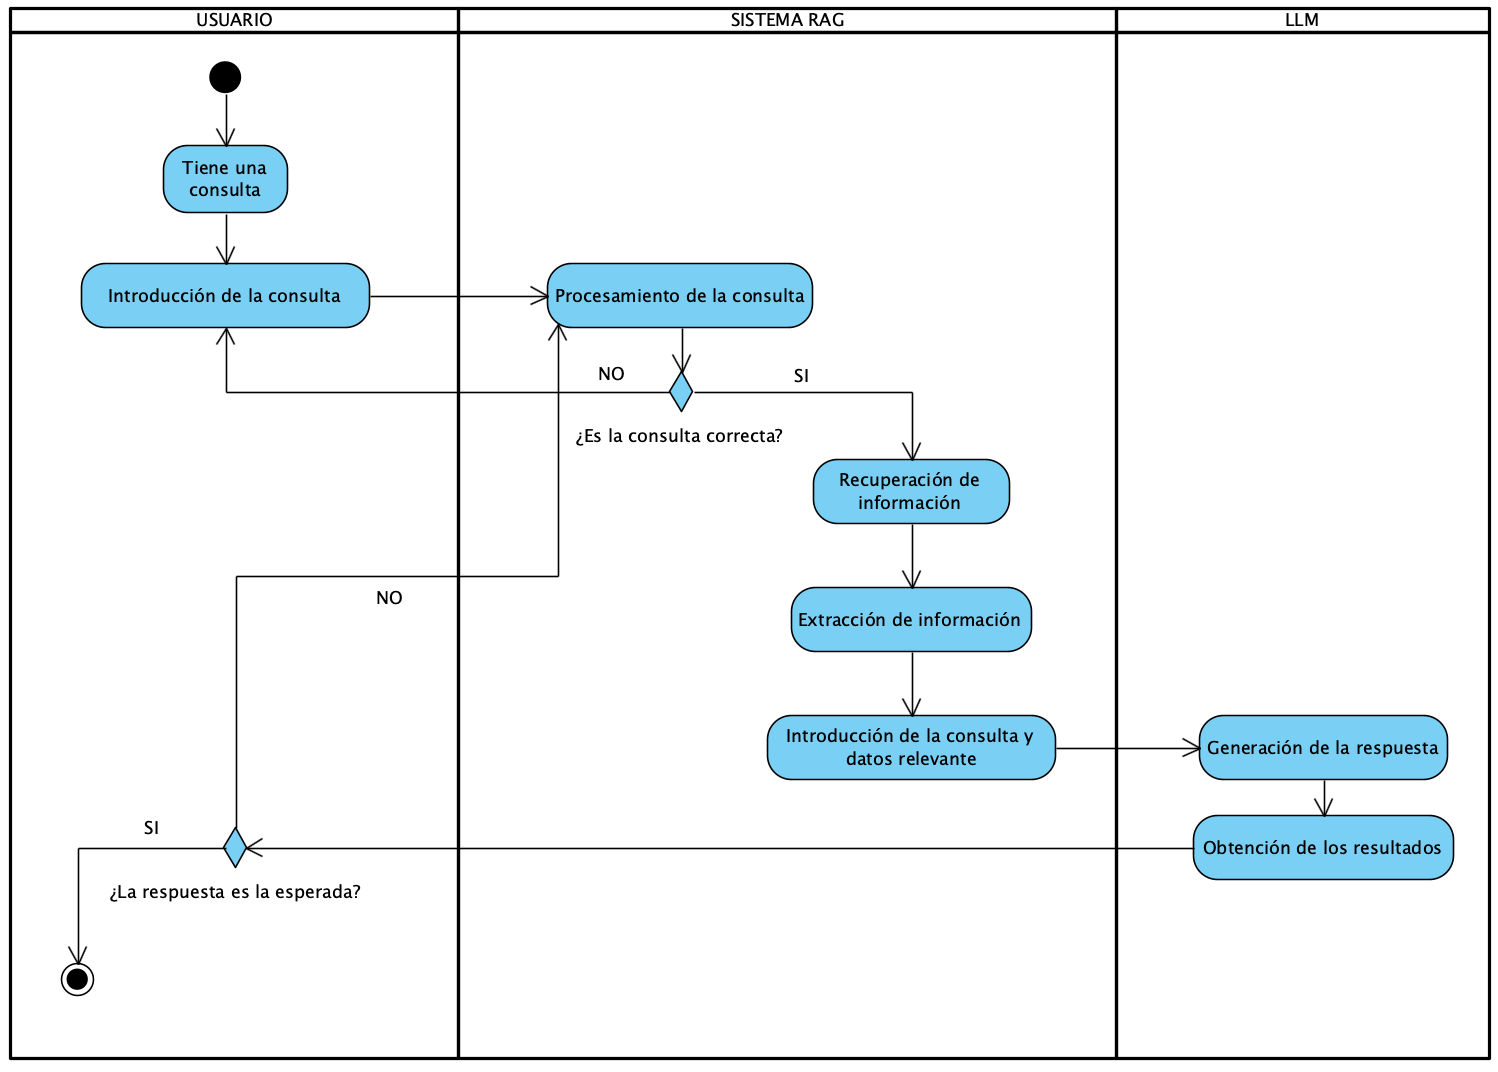
\includegraphics[width=0.8\textwidth]{TFGDocumentacion-master/imagenes/DiagramaActividadRAG.png}
    \caption{Diagrama de actividad del sistema RAG.}
    \label{Fig.DiagramAct}
\end{figure}





